\documentclass[oneside,14pt]{extarticle}
\usepackage{cmap}
\usepackage[utf8]{inputenc}
\usepackage[english,ukrainian]{babel}
\usepackage{graphicx}
\usepackage{geometry}
\usepackage{listings}
\usepackage{float}
\usepackage{amsmath}
\usepackage{subfig}
\usepackage{tempora}
\geometry{
	a4paper,
	left=20mm,
	right=20mm,
	top=15mm,
	bottom=15mm,
}
\lstset{
	language=c,
	tabsize=4,
	keepspaces,
	showstringspaces=false,
	frame=single,
	breaklines,
	language=C,
}
\graphicspath{ {./pictures} }
\setlength{\parindent}{4em}

\newcommand\subject{Системне адміністрування}
\newcommand\lecturer{професор кафедри ПЗ\\Фечан А.В.}
\newcommand\teacher{професор кафедри ПЗ\\Фечан А.В.}
\newcommand\mygroup{ПЗ-42}
\newcommand\lab{1}
\newcommand\theme{Управління дисками в Windows 10, створення програмних
	RAID-масивів}
\newcommand\purpose{Вивчити принципи роботи файлових систем FAT та NTFS в
	ОС Windows 10; навчитись управляти дисковим простором та створювати
	програмні RAID масиви на динамічних дисках у Windows 10}

\begin{document}
\begin{normalsize}
	\begin{titlepage}
		\thispagestyle{empty}
		\begin{center}
			\textbf{МІНІСТЕРСТВО ОСВІТИ І НАУКИ УКРАЇНИ\\
				НАЦІОНАЛЬНИЙ УНІВЕРСИТЕТ "ЛЬВІВСЬКА ПОЛІТЕХНІКА"}
		\end{center}
		\begin{flushright}
			\textbf{ІКНІ}\\
			Кафедра \textbf{ПЗ}
		\end{flushright}
		\vspace{80pt}
		\begin{center}
			\textbf{ЗВІТ}\\
			\vspace{10pt}
			до лабораторної роботи № \lab\\
			\textbf{на тему}: <<\textit{\theme}>>\\
			\textbf{з дисципліни}: <<\subject>>
		\end{center}
		\vspace{80pt}
		\begin{flushright}
			
			\textbf{Лектор}:\\
			\lecturer\\
			\vspace{28pt}
			\textbf{Виконав}:\\
			
			студент групи \mygroup\\
			Коваленко Д.М.\\
			\vspace{28pt}
			\textbf{Прийняв}:\\
			
			\teacher\\
			
			\vspace{28pt}
			«\rule{1cm}{0.15mm}» \rule{1.5cm}{0.15mm} 2024 р.\\
			$\sum$ = \rule{1cm}{0.15mm}……………\\
			
		\end{flushright}
		\vspace{\fill}
		\begin{center}
			\textbf{Львів — 2024}
		\end{center}
	\end{titlepage}
		
	\begin{description}
		\item[Тема.] \theme.
		\item[Мета.] \purpose.
	\end{description}

    \section*{Лабораторне завдання}
	\begin{enumerate}
		\item Створити розширений розділ на першому жорсткому диску (рис. 1);
		створити 3 логічні диски в цьому розділі – файлова система FAT 32, розмір
		кластера 512 байт, 8 кБ, та 64 кБ відповідно.
		\item Скопіювати папку, що містить велику кількість файлів невеликого
		розміру на кожен з цих томів. Порівняти реальний
		розмір цієї папки на кожному томі.
		\item Конвертувати файлову систему на цих томах в NTFS
		використовуючи утиліту convert.exe.
		\item Створити на томі з файловою системою NTFS файл розміром 500–
		600 байт (наприклад текстовий документ). Переконатися, що кількість
		вільного/зайнятого місця на томі не змінилась.
		\item Створити на томі з ФС NTFS порожній файл. Записати якусь
		інформацію в іменований потік цього файлу (наприклад за допомогою команди
		echo або перенаправлення виводу іншого файлу в цей потік). Переконатись, що хоча вільне місце на томі відображається коректно, розмір
		файлу "залишається" нульовим (незмінним).
		\item За допомогою оснастки «Керування дисками» перетворити базові диски
		в динамічні.
		\item Створити на динамічних дисках простий, складений та почерговий томи.
		Розширити простий том в межах одного диску. Розширити цей же том на інший
		диск; звернути увагу на тип тому, що утворився в результаті цієї операції.
	\end{enumerate}

	\section*{Хід роботи}
	
	\begin{figure}[H]
		\centering
		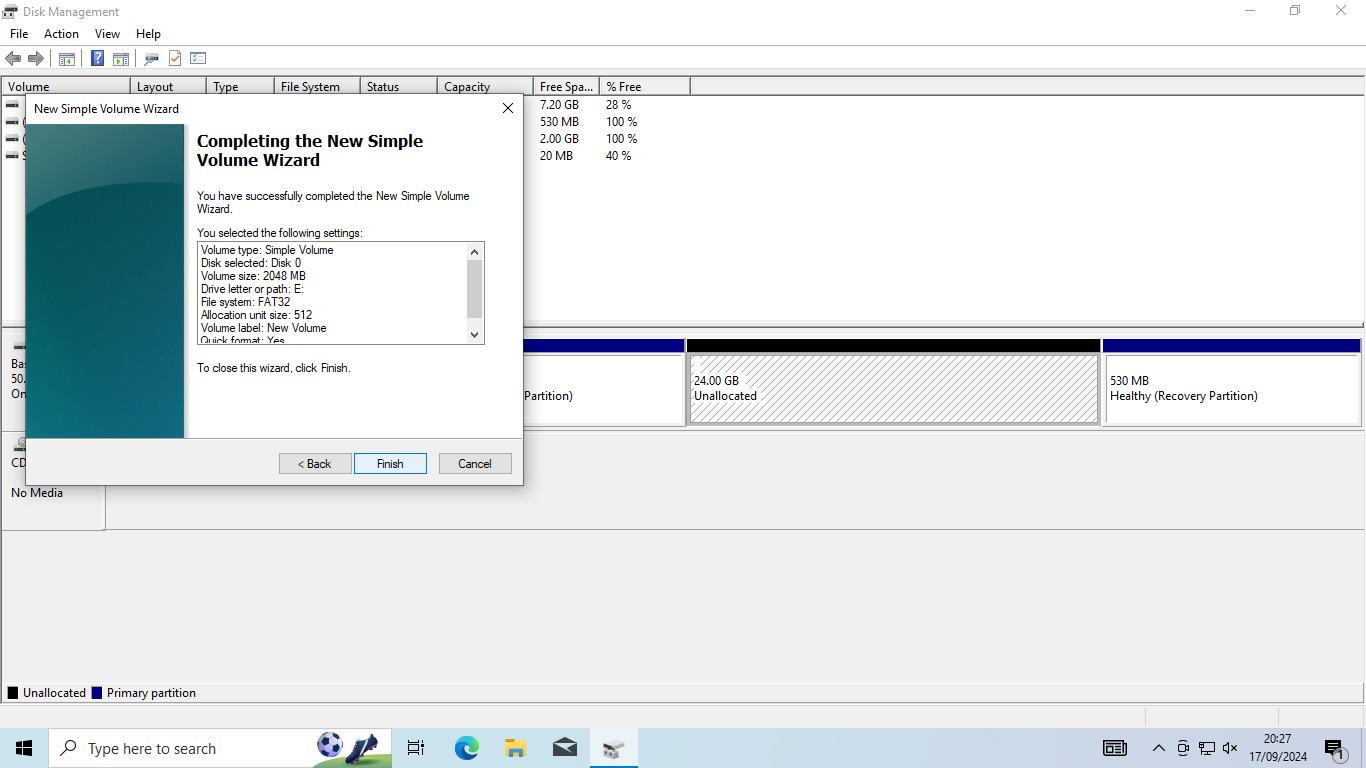
\includegraphics[scale=0.4]{1}
		\caption{Створення розділу з файловою системою FAT 32, розмір кластера 512 байт}
	\end{figure}
	
	\begin{figure}[H]
		\centering
		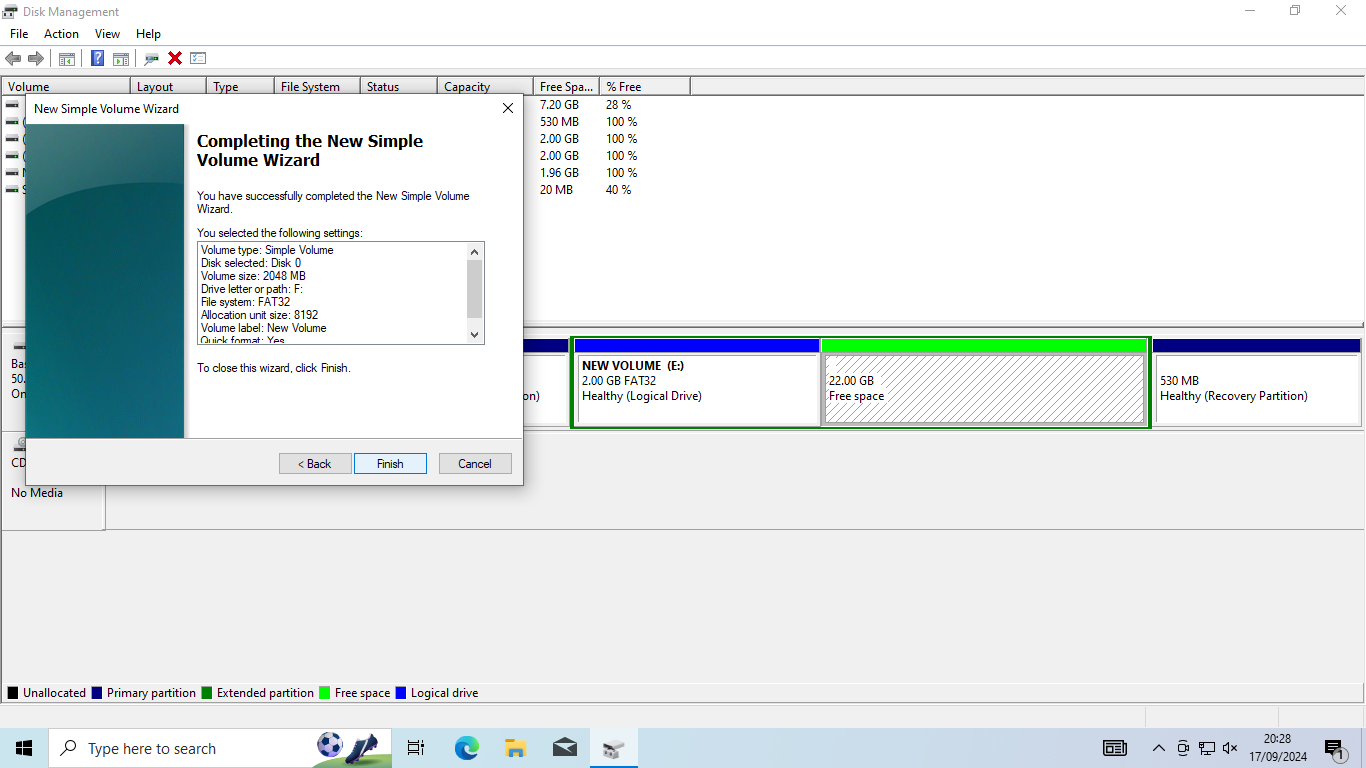
\includegraphics[scale=0.4]{2}
		\caption{Створення розділу з файловою системою FAT 32, розмір кластера 8 кБ}
	\end{figure}
	
	\begin{figure}[H]
		\centering
		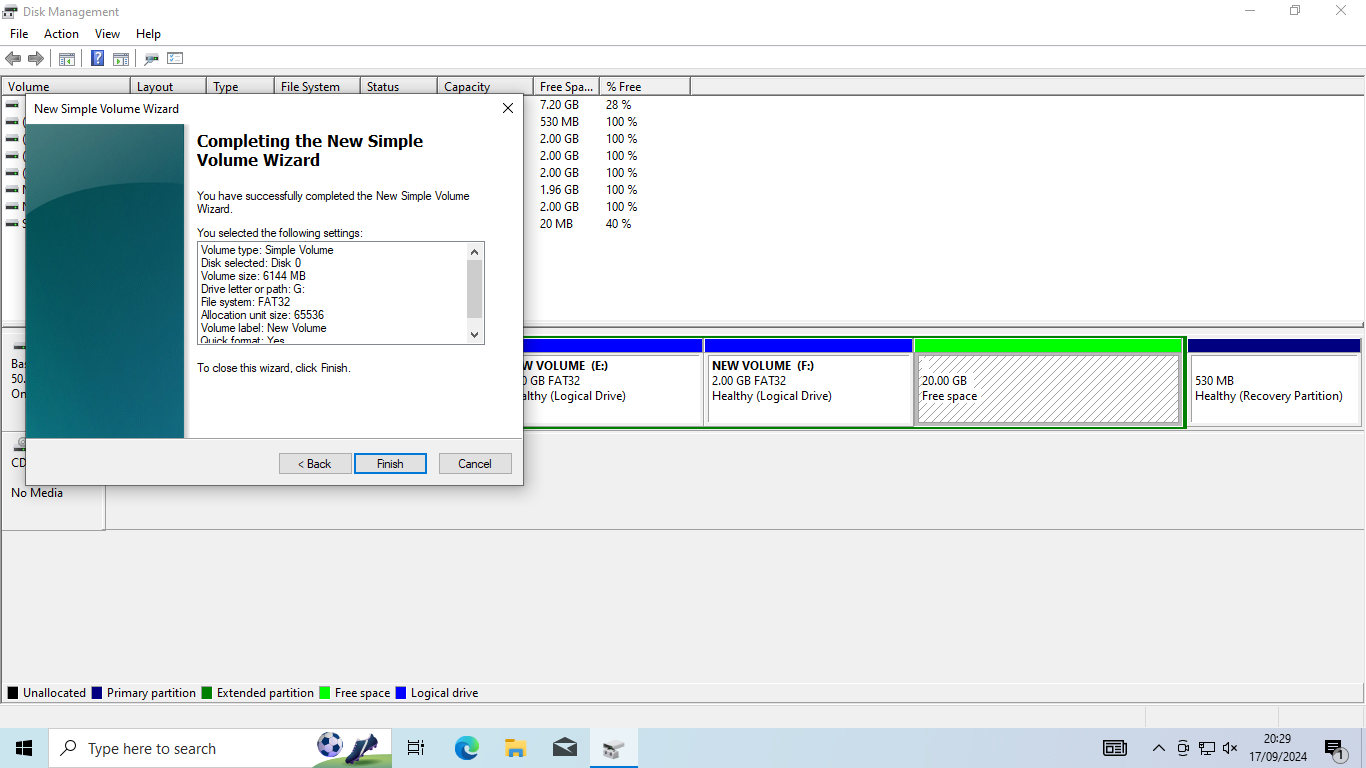
\includegraphics[scale=0.4]{3}
		\caption{Створення розділу з файловою системою FAT 32, розмір кластера 64 кБ}
	\end{figure}
	
	\begin{figure}[H]
		\centering
		\begin{minipage}{0.3\textwidth}
			\centering
			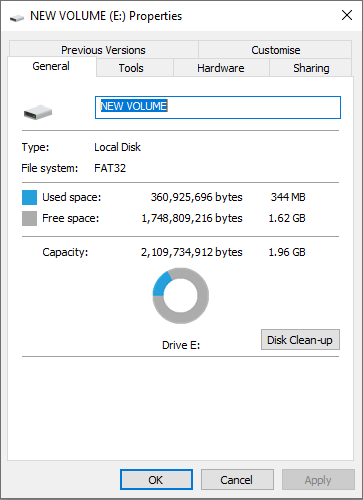
\includegraphics[scale=0.5]{4}
			\caption*{Розмір кластера 512 б}
		\end{minipage}
		\hfill
		\begin{minipage}{0.3\textwidth}
			\centering
			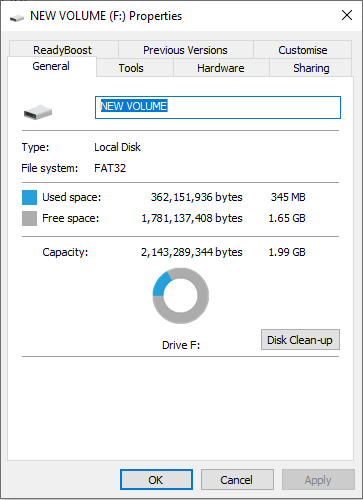
\includegraphics[scale=0.5]{5}
			\caption*{Розмір кластера 8 кБ}
		\end{minipage}
		\hfill
		\begin{minipage}{0.3\textwidth}
			\centering
			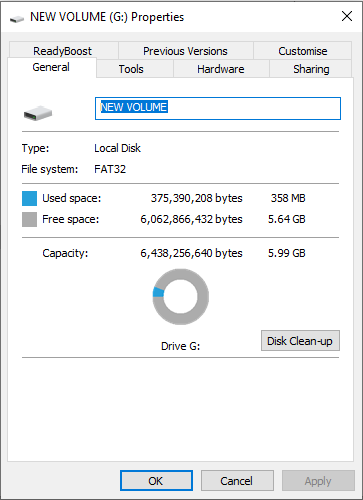
\includegraphics[scale=0.5]{6}
			\caption*{Розмір кластера 64 кБ}
		\end{minipage}
		\caption{Кількість місця, що займає папка на диску, залежно від розміру кластера}	
	\end{figure}
	
	\begin{figure}[H]
		\centering
		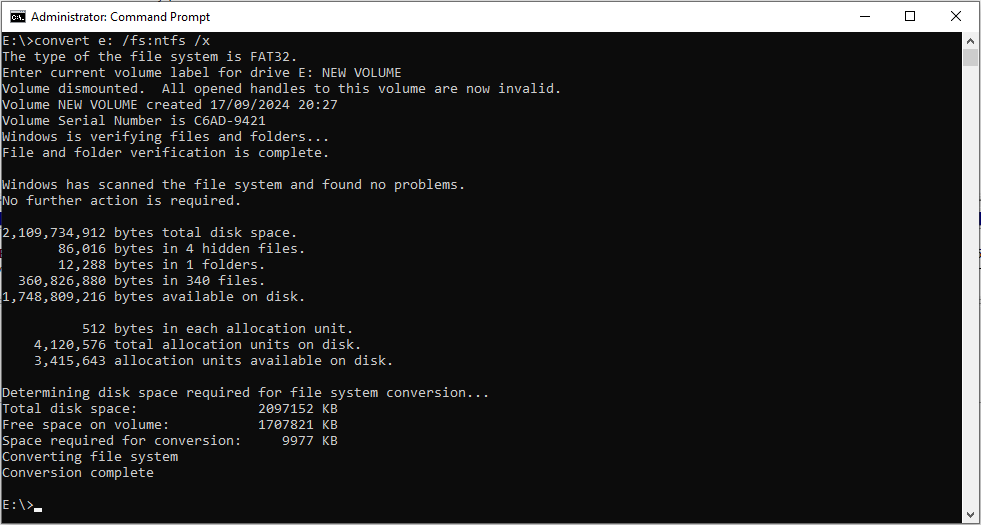
\includegraphics[scale=0.5]{7}
		\caption{Конвертація розділу у файлову систему NTFS за допомогою утиліти convert.exe, розмір кластера 512 байт}
	\end{figure}
	
	\begin{figure}[H]
		\centering
		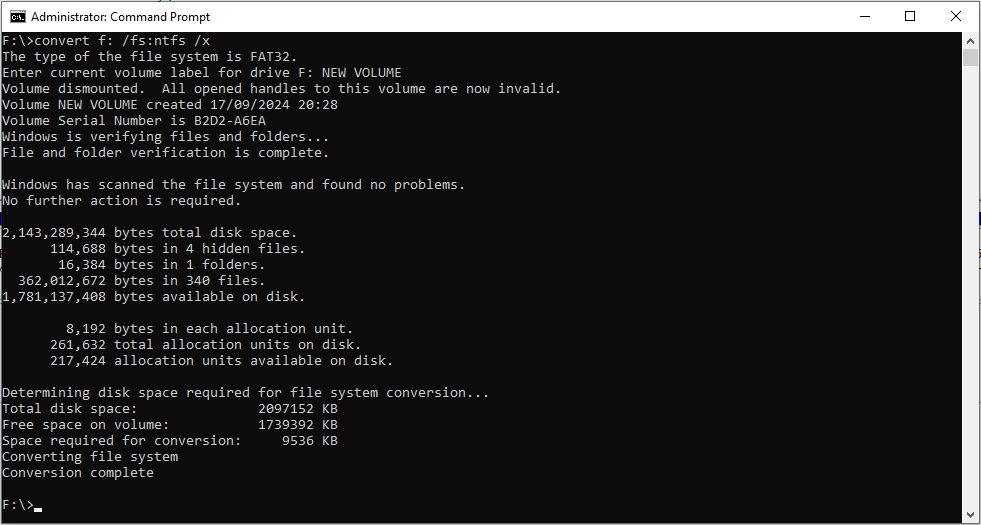
\includegraphics[scale=0.5]{8}
		\caption{Конвертація розділу у файлову систему NTFS за допомогою утиліти convert.exe, розмір кластера 8 кБ}
	\end{figure}
	
	\begin{figure}[H]
		\centering
		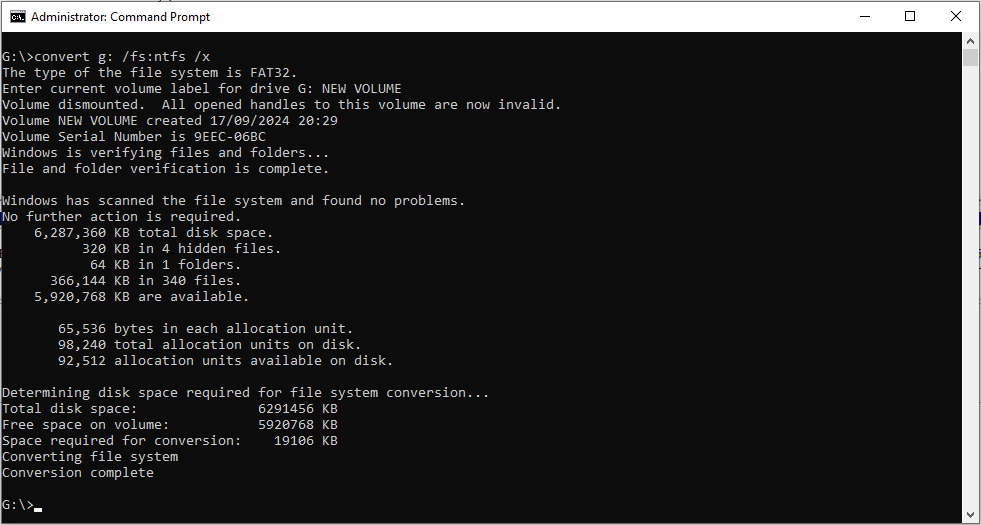
\includegraphics[scale=0.5]{9}
		\caption{Конвертація розділу у файлову систему NTFS за допомогою утиліти convert.exe, розмір кластера 64 кБ}
	\end{figure}
	
	\begin{figure}[H]
		\centering
		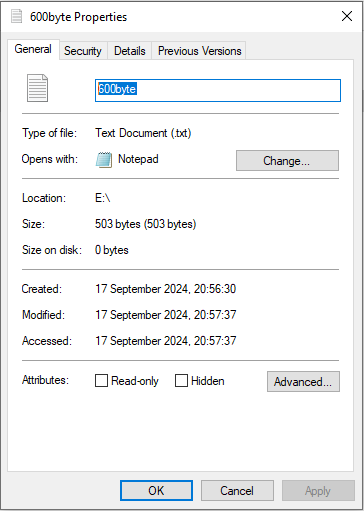
\includegraphics[scale=0.6]{10}
		\caption{Демонстрація файлу розміром 500 байт, що не займає місця на диску}
	\end{figure}
	
	\begin{figure}[H]
		\centering
		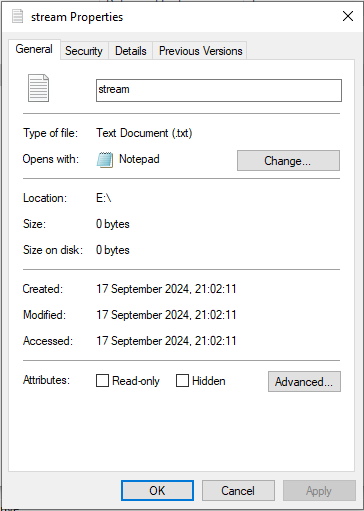
\includegraphics[scale=0.6]{11}
		\caption{Демонстрація файлу з іменованими потоками NTFS}
	\end{figure}
	
	\begin{figure}[H]
		\centering
		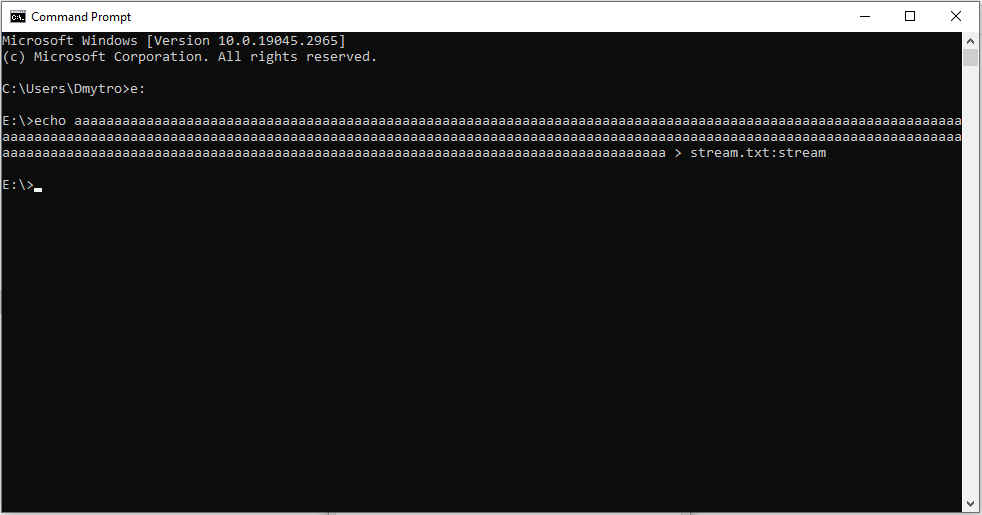
\includegraphics[scale=0.5]{12}
		\caption{Демонстрація використання іменованих потоків NTFS}
	\end{figure}
	
	\begin{figure}[H]
		\centering
		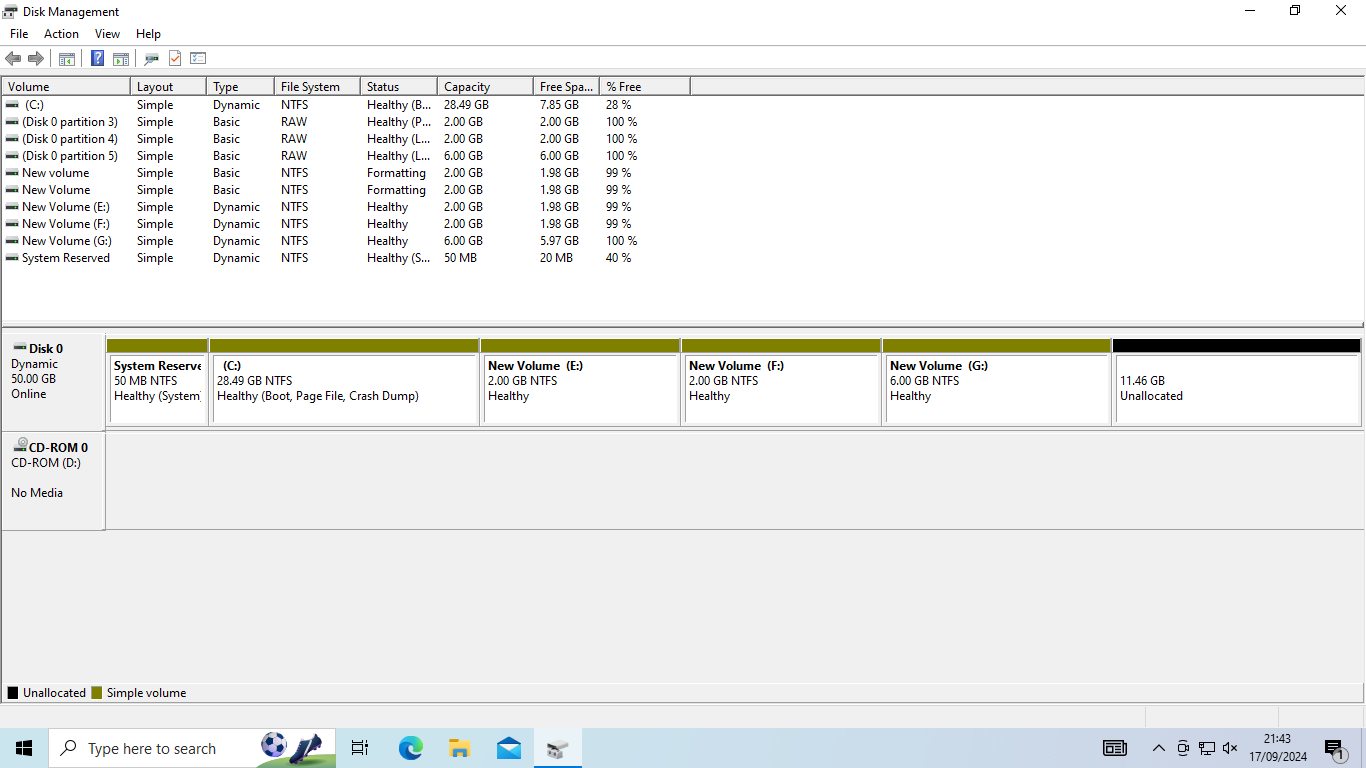
\includegraphics[scale=0.4]{13}
		\caption{Результат перетворення дисків на динамічні}
	\end{figure}
	
	\begin{figure}[H]
		\centering
		\begin{minipage}{0.45\textwidth}
			\centering
			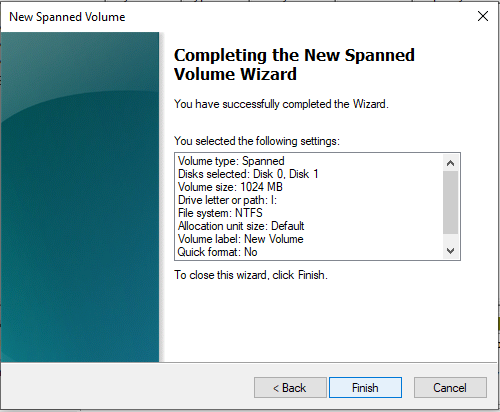
\includegraphics[scale=0.6]{14}
			\caption{Створення складеного тому}
		\end{minipage}
		\hfill
		\begin{minipage}{0.45\textwidth}
			\centering
			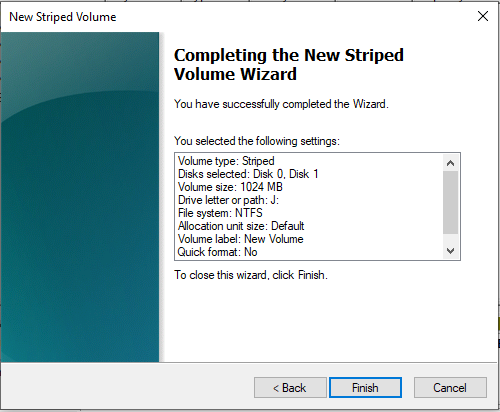
\includegraphics[scale=0.6]{15}
			\caption{Створення почергового тому}
		\end{minipage}
	\end{figure}
	
	Під час розширення простого тому на інший диск, його тип було змінено на складений.
	
	\begin{figure}[H]
		\centering
		\begin{minipage}{0.45\textwidth}
			\centering
			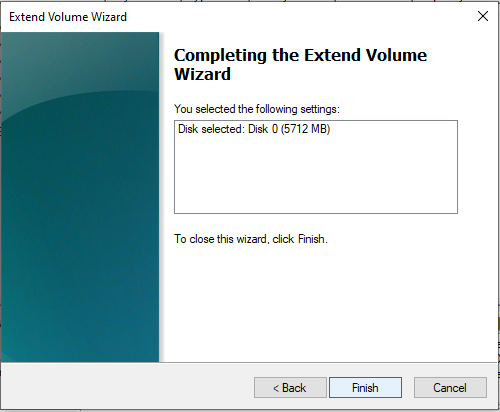
\includegraphics[scale=0.6]{16}
			\caption{Розширення простого тому в межах диску}
		\end{minipage}
		\hfill
		\begin{minipage}{0.45\textwidth}
			\centering
			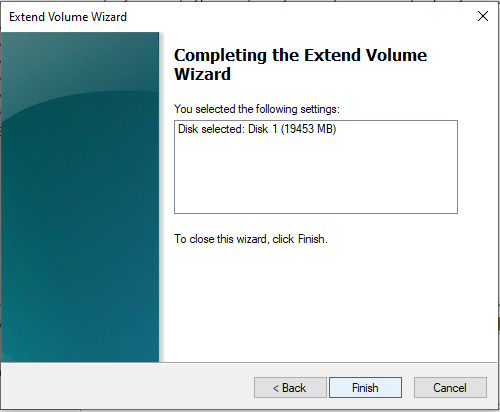
\includegraphics[scale=0.6]{17}
			\caption{Розширення простого тому на інши диск}
		\end{minipage}
	\end{figure}
	
	\begin{figure}[H]
		\centering
		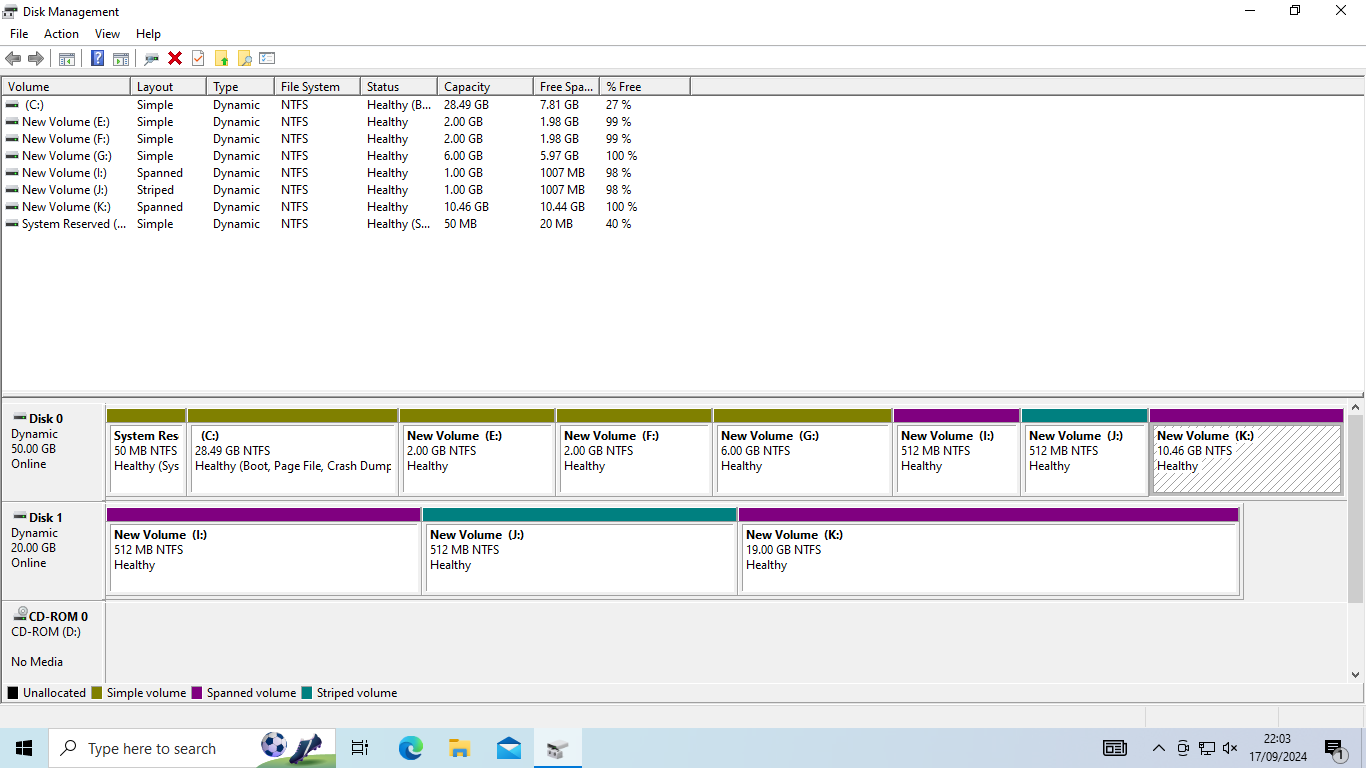
\includegraphics[scale=0.4]{18}
		\caption{Результат}
	\end{figure}
	
	\section*{Висновки}
	Під час виконання лабораторної роботи я вивчив принципи роботи файлових систем FAT та NTFS в
	ОС Windows 10; навчився управляти дисковим простором та створювати
	програмні RAID масиви на динамічних дисках у Windows 10
		    
\end{normalsize}
\end{document}
